\documentclass{beamer}
\usetheme{Madrid}
\usecolortheme{default}
\usepackage{tikz}
\usetikzlibrary{shapes.geometric, arrows, positioning}

\title[Advanced WAF]{Advanced Web Application Firewall (WAF) Architecture}
\subtitle{Implementation using Rabin-Karp \& 3-Layer Defense System}
\author[Team]{
    Sneha Singh - 231081067 \\
    Jay Ghorpade - 231080026 \\
    Kajal Kumari - 231081034
}
\institute{Cybersecurity Lab}
\date{\today}

\begin{document}

\frame{\titlepage}

\begin{frame}
\frametitle{Introduction}
\textbf{The Problem with "Basic" WAFs:}
\begin{itemize}
    \item Traditional basic WAFs rely solely on simple string matching and primitive regex rules.
    \item High rate of false positives and high performance overhead ($O(n \times m)$).
    \item Easily bypassed using payload obfuscation (e.g., URL or HTML encoding).
\end{itemize}
\vspace{0.4cm}
\textbf{Our Solution: Beyond a "Basic Project"}
\begin{itemize}
    \item \textbf{Algorithmic Approach:} Implements the \textbf{Rabin-Karp Algorithm} (rolling hashes) for high-speed signature matching.
    \item \textbf{Resilience against Obfuscation:} Uses an integrated sanitizer pipeline.
    \item \textbf{Hybrid Architecture:} A 3-Layer Defense mechanism ensuring both performance and accuracy against SQLi and XSS.
\end{itemize}
\end{frame}

\begin{frame}
\frametitle{System Architecture: 3-Layer Defense Flowchart}
\begin{center}
\resizebox{0.9\textwidth}{!}{%
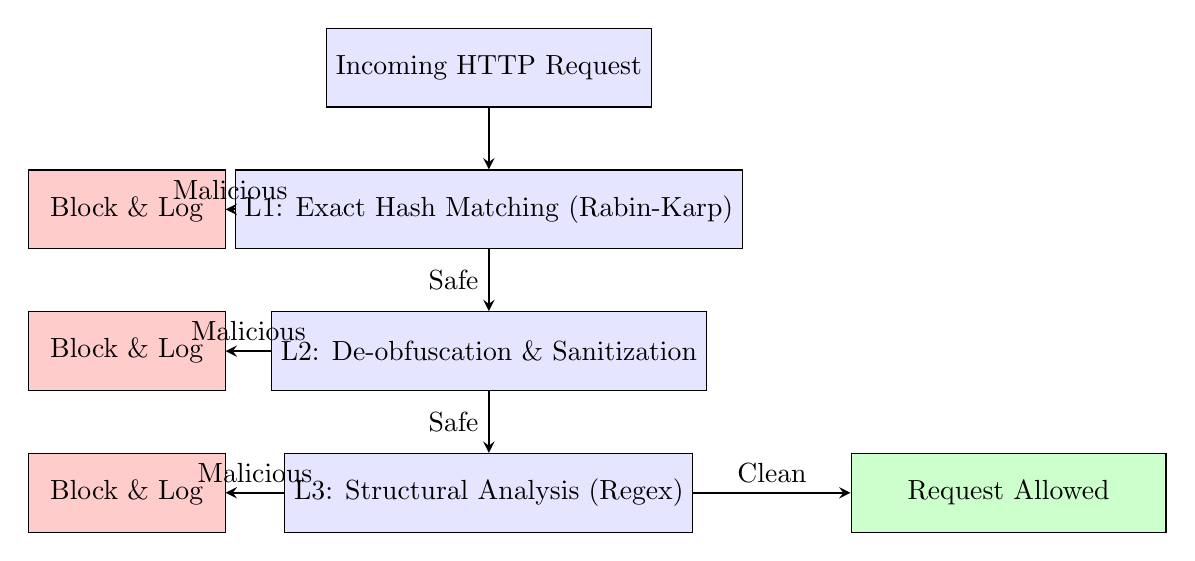
\begin{tikzpicture}[node distance=1.6cm]
\tikzstyle{process} = [rectangle, minimum width=4cm, minimum height=1cm, text centered, draw=black, fill=blue!10]
\tikzstyle{arrow} = [thick,->,>=stealth]
\tikzstyle{alert} = [rectangle, minimum width=2.5cm, minimum height=1cm, text centered, draw=black, fill=red!20]

\node (input) [process] {Incoming HTTP Request};
\node (l1) [process, below of=input, yshift=-0.2cm] {L1: Exact Hash Matching (Rabin-Karp)};
\node (l2) [process, below of=l1, yshift=-0.2cm] {L2: De-obfuscation \& Sanitization};
\node (l3) [process, below of=l2, yshift=-0.2cm] {L3: Structural Analysis (Regex)};
\node (pass) [process, fill=green!20, right of=l3, xshift=5cm] {Request Allowed};

\node (block1) [alert, left of=l1, xshift=-3cm] {Block \& Log};
\node (block2) [alert, left of=l2, xshift=-3cm] {Block \& Log};
\node (block3) [alert, left of=l3, xshift=-3cm] {Block \& Log};

\draw [arrow] (input) -- (l1);
\draw [arrow] (l1) -- node[anchor=east] {Safe} (l2);
\draw [arrow] (l1) -- node[anchor=south] {Malicious} (block1);

\draw [arrow] (l2) -- node[anchor=east] {Safe} (l3);
\draw [arrow] (l2) -- node[anchor=south] {Malicious} (block2);

\draw [arrow] (l3) -- node[anchor=south] {Malicious} (block3);
\draw [arrow] (l3) -- node[anchor=south] {Clean} (pass);

\end{tikzpicture}
}
\end{center}
\end{frame}

\begin{frame}
\frametitle{Layer 1: Rabin-Karp Hash Matching}
\textbf{Why Rabin-Karp?}
\begin{itemize}
    \item \textbf{Performance:} Utilizes a rolling hash to check payloads in $O(n+m)$ average time, compared to $O(n \times m)$ of naive substring matching.
    \item \textbf{Algorithm Design:}
    \begin{itemize}
        \item Base = 256, Modulo = 101.
        \item Quickly scans incoming HTTP data (headers, query parameters, body) for known exact malicious signatures (e.g., \texttt{UNION}, \texttt{DROP}, \texttt{<script>}).
    \end{itemize}
    \item \textbf{Impact:} Eliminates the need to evaluate heavy Regular Expressions on every request, drastically reducing CPU overhead on safe traffic and guaranteeing minimal latency.
\end{itemize}
\end{frame}

\begin{frame}
\frametitle{Layer 2: Payload De-obfuscation}
\textbf{Defeating Modern Evasion Techniques}
\begin{itemize}
    \item Attackers frequently attempt to bypass basic filters by obfuscating payloads:
    \begin{itemize}
        \item \textit{Example:} \texttt{\%27\%20OR\%20\%271\%27\%3D\%271} (URL Encoded SQLi)
    \end{itemize}
    \vspace{0.2cm}
    \item \textbf{Sanitizer Module Operations:}
    \begin{itemize}
        \item Normalizes request data before it reaches the final Regex checks.
        \item Handles comprehensive decoding: URL-encoding, HTML entities, and Unicode escapes.
    \end{itemize}
    \item \textbf{Re-evaluation Loop:} Once decoded, the payload is recursively passed through the detection engines to ensure hidden attacks are successfully neutralized.
\end{itemize}
\end{frame}

\begin{frame}
\frametitle{Layer 3: Structural Threat Recognition (Regex)}
\textbf{Handling Evolving \& Complex Attacks}
\begin{itemize}
    \item Exact keyword matching (Layer 1) cannot catch everything due to extreme syntax variations and specific logic injections.
    \item \textbf{Regex Fallback:}
    \begin{itemize}
        \item Scans for structural anomalies that signify Logic Errors or code injection.
        \item \textit{Example SQLi Pattern:} \texttt{('\textbackslash s*(or|and)\textbackslash s*'?\textbackslash d)}
        \item \textit{Example XSS Pattern:} Structural checking for injecting malicious handlers like \texttt{onerror=} or \texttt{javascript:}.
    \end{itemize}
    \item \textbf{Summary:} Balances the need for exact pattern recognition (Rabin-Karp) with the flexibility required to catch unknown, syntactical variants.
\end{itemize}
\end{frame}

\begin{frame}
\frametitle{Defensive Logging \& Analytics}
\textbf{Complete Threat Transparency}
\begin{itemize}
    \item Beyond simple blocking, our WAF acts as an analytical tool, intercepting and logging detailed threat intelligence.
    \item \textbf{Metrics Tracked:}
    \begin{itemize}
        \item \textbf{Layer Effectiveness:} Logs which specific layer (Hash vs Regex) intercepted the attack.
        \item \textbf{Collision Tracking:} Captures "spurious hits" to evaluate and tune the Rabin-Karp hashing modulo.
        \item \textbf{Execution Metrics:} Logs exact pattern matching comparisons to demonstrate absolute efficiency over naive matching.
    \end{itemize}
\end{itemize}
\end{frame}

\begin{frame}
\frametitle{Conclusion \& Future Scope}
\begin{itemize}
    \item \textbf{Summary:}
    \begin{itemize}
        \item Successfully engineered an advanced Web Application Firewall that merges foundational Data Structures (Rolling Hashes) with Applied Cybersecurity.
        \item Built a pipeline that defeats obfuscation and ensures scalability.
    \end{itemize}
    \vspace{0.3cm}
    \item \textbf{Future Enhancements:}
    \begin{itemize}
        \item Integrate Machine Learning (e.g., Naive Bayes or LSTM models) to dynamically identify zero-day vulnerabilities.
        \item Implement IP-based Rate Limiting to mitigate specific Denial of Service (DoS) and Brute-Force attacks.
    \end{itemize}
\end{itemize}
\vspace{0.5cm}
\begin{center}
    \textbf{Thank You! \\ Questions?}
\end{center}
\end{frame}
\end{document}
